\documentclass[11pt]{article}
\usepackage[bordered]{uni-style}
\usepackage{wrapfig}
\usepackage{capt-of}
\usepackage{multicol}
\title{آزمایشگاه ساختار کامپیوتر و میکروپروسسور}
\prof{دکتر باقری شورکی}
\subtitle{آشنایی با منابع وقفه 8051}
\subject{ گزارش آزمایش هشتم}
\department{مهندسی برق}
\info{
    \begin{tabular}{rl}
        برنا خدابنده & 400109898\\
    \end{tabular}
}
\date{\today}
\usepackage{xepersian}
\settextfont{Yas}

\newcommand*{\question}[1]{
	\vspace*{-1em}
	\begin{figure}[h]
		\centering
		\includegraphics[width=0.95\linewidth]{question/#1}
	\end{figure}
}

\begin{document}
\maketitlepage
\maketitlestart

\section{پرسش اول}

هدف از این آزمایش بررسی نحوه ی ارتباط سریال آسنکرون (UART (توسط
میکروکنترلر 8051 است. از پروتکل UART برای ارتباط سریال بین دو دستگاه استفاده می
شود، به این صورت که فرستنده دیتا را به صورت موازی می گیرد سپس آن را سریال می
کند و از طریق پورت Tx خود دیتای سریال شده را به گیرنده می فرستد. گیرنده دیتای
سریال شده را از پورت Rx دریافت می کند و بعد از اتمام دریافت آن را موازی می کند .
دیتاها از طریق UART به صورت بسته منتقل می شوند یعنی اینکه ابتدا یک بیت برای شروع
فرستاده می شود، سپس تعدادی بیت به عنوان دیتا و سپس یک یا دو بیت نشان دهنده ی
پایان بسته فرستاده می شود. برای مثال اگر بیت شروع را به صورت قرار داد صفر بگیریم
تا زمانی که دیتایی نمی فرستیم بیت یک ارسال می شود ولی به محض اینکه بیت صفر ارسال
شود گیرنده متوجه می شود که مثال 8 بیت بعدی دیتا هستند. با توجه به آسنکرون بودن
ارتباط )نیاز به فرستادن کالک همراه با دیتا نمی باشد( باید هر دو دستگاه در یک سرعت
کار کنند که به آن baudrate گفته می شود. در مورد baudrate بیشتر تحقیق کنید، تفاوت
آن با (bitrate (چیست؟ 

\subsection{\lr{bitrate-baudrate}}

حالا، درباره تفاوت بین نرخ بیت و نرخ بود صحبت کنیم:

\begin{itemize}
	\item \textbf{bitrate : } نرخ بیت به تعداد بیت‌های ارسالی در واحد زمان اشاره دارد. این نرخ نشان‌دهنده سرعت ارسال داده در یک کانال ارتباطی است و به بیت در ثانیه (bps) اندازه‌گیری می‌شود. به عنوان مثال، نرخ بیت ۹۶۰۰ bps به این معنی است که ۹۶۰۰ بیت از داده‌ها در یک ثانیه ارسال یا دریافت می‌شوند.
	\item \textbf{baudrate : } به تعداد تغییرات سیگنال در ثانیه در یک کانال ارتباطی اشاره دارد. این نرخ تعداد تغییرات نمادها (مودولاسیون یا رویدادهای سیگنال) را نشان می‌دهد که در هر ثانیه رخ می‌دهد و به بودها یا نمادها در ثانیه (bauds) اندازه‌گیری می‌شود.
\end{itemize}

در استاندارد RS-232، به طور معمول هر نماد نشان‌دهنده یک بیت داده است. بنابراین، باود ریت اغلب به طور معادل با نرخ بیت استفاده می‌شود. با این حال، در برخی از روش‌های مودولاسیون که چندین بیت در یک نماد رمزگذاری می‌شوند، نرخ بود و نرخ بیت ممکن است متفاوت باشند.


\begin{figure}[h!]
	\centering
	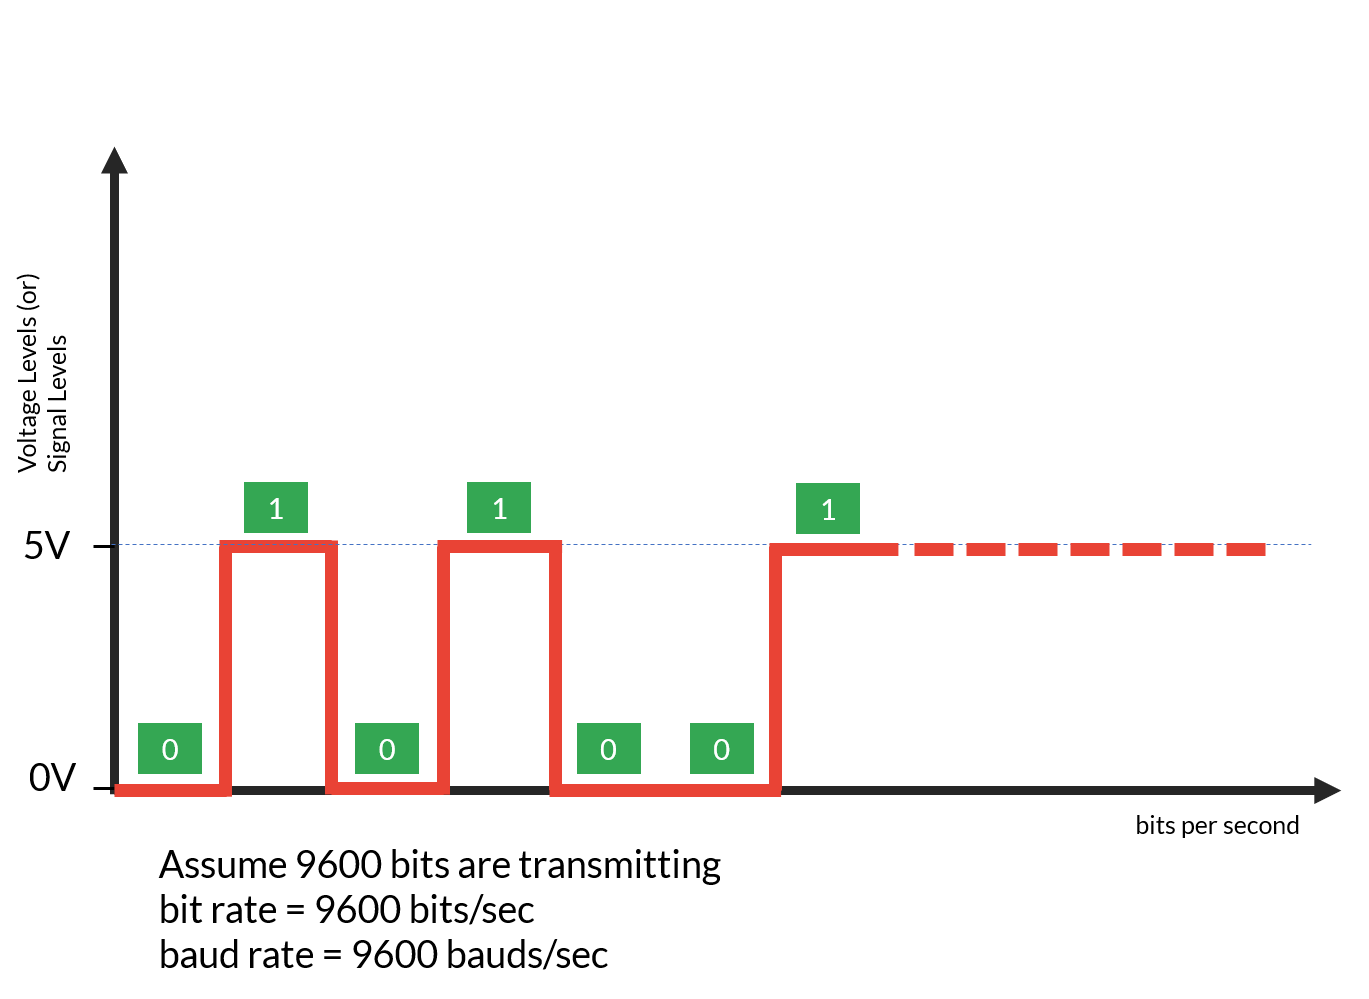
\includegraphics[height=5.5cm]{result/Bitrateequalbaudrate.png}
\end{figure}


پورت سریال ،8051 duplex Full می باشد، به این معنی که همزمان هم میتوان دیتا
فرستاد و هم میتوان دریافت کرد. دو پین جداگانه TXD و RXD برای این منظور وجود
دارد.
) TXD پین 3.1p می باشد و RXD پین 3.0p می باشد( . رجیستر مخصوص ارتباط سریال
SBUF می باشد که با استفاده از MOV می توان دیتا را بر روی آن قرار داد یا از آن خواند .

\clearpage

\subsection{قسمت الف}

 برنامه ای بنویسید که عدد 42H را به طور مداوم به خروجی ارسال نماید. سیگنال
خروجی را بر روی اسیلوسکوپ مشاهده نمایید. بر اساس اندازه گیری زمان پالس ها،
فرکانس کالک سیستم و baudrate را به دست آورید.)از مود 0 استفاده کنید)


\begin{qsolve}[]
	کد زیر را در نظر بگیرید.
	\begin{latin}
		\begin{verbatim}
			ORG 0000H            ; Set the origin address of the program
			
			START:              
				MOV TMOD, #00H    ; Configure Timer 0 and Timer 1 in 13-bit mode
				MOV TH1, #0F0H    ; Set the baud rate for serial communication
				MOV IE, #88H      ; Enable Timer 1 and Serial Port interrupts
				SETB TR1          ; Start Timer 1
				
			MAIN:               ; Main program loop
				MOV A, #4        ; Load the value 4 into the accumulator
				CALL SEND        ; Call the SEND subroutine to send the value
				MOV A, #2        ; Load the value 2 into the accumulator
				CALL SEND        ; Call the SEND subroutine again to send the new value
				JMP MAIN         ; Jump back to the beginning of the main loop
				
			SEND:               ; Subroutine for sending data via the serial port
				MOV SCON, #00H   ; Configure the serial port in mode 0
				MOV SBUF, A      ; Move the value in the accumulator to the serial data buffer
			WAIT:               ; Loop to wait for transmission completion
				JNB TI, WAIT     ; Jump to WAIT if the transmit interrupt flag is not set
				CLR TI           ; Clear the transmit interrupt flag
				RET              ; Return from the subroutine
		\end{verbatim}
	\end{latin}

	 با این کد، با استفاده از تایمر برای زمان بندی و مود 0 ارتباط سریال، عدد هکس \texttt{H42} را 
	 ارسال میکنیم.

	 \begin{center}
		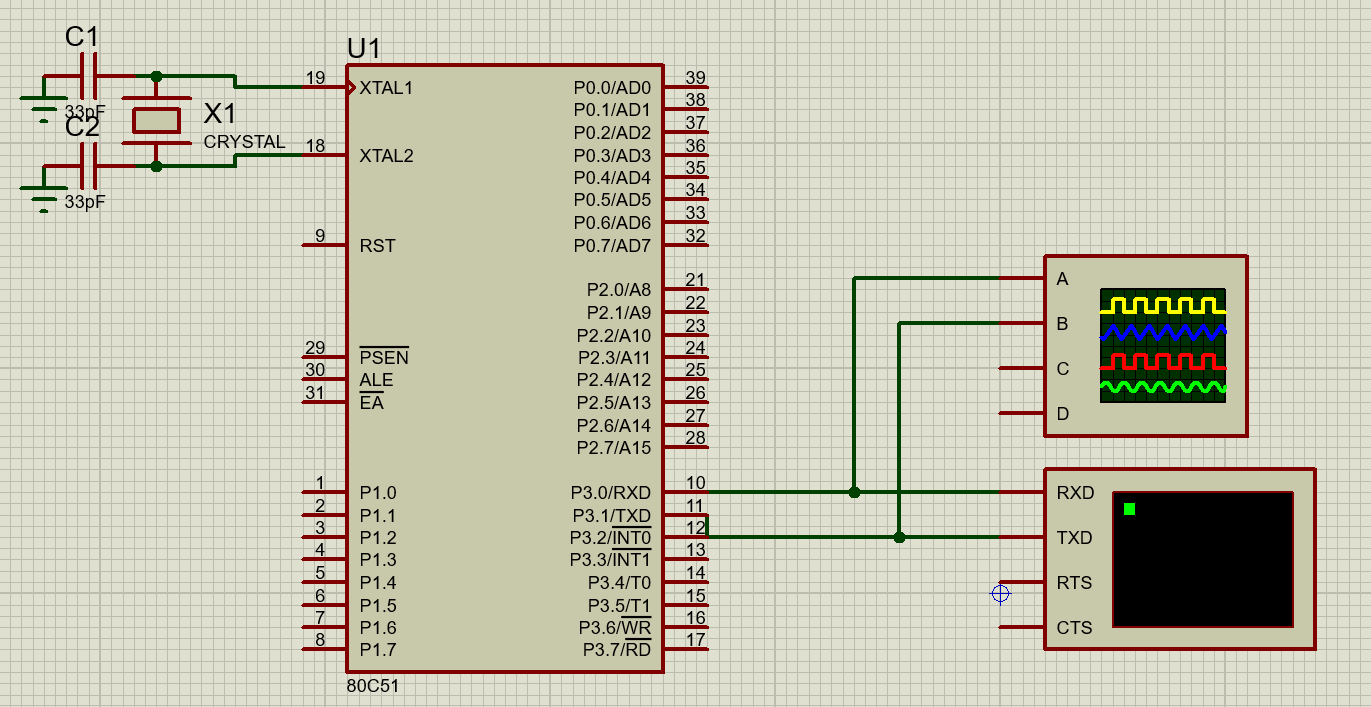
\includegraphics[width=0.48\linewidth]{result/p1_proteus.png}
		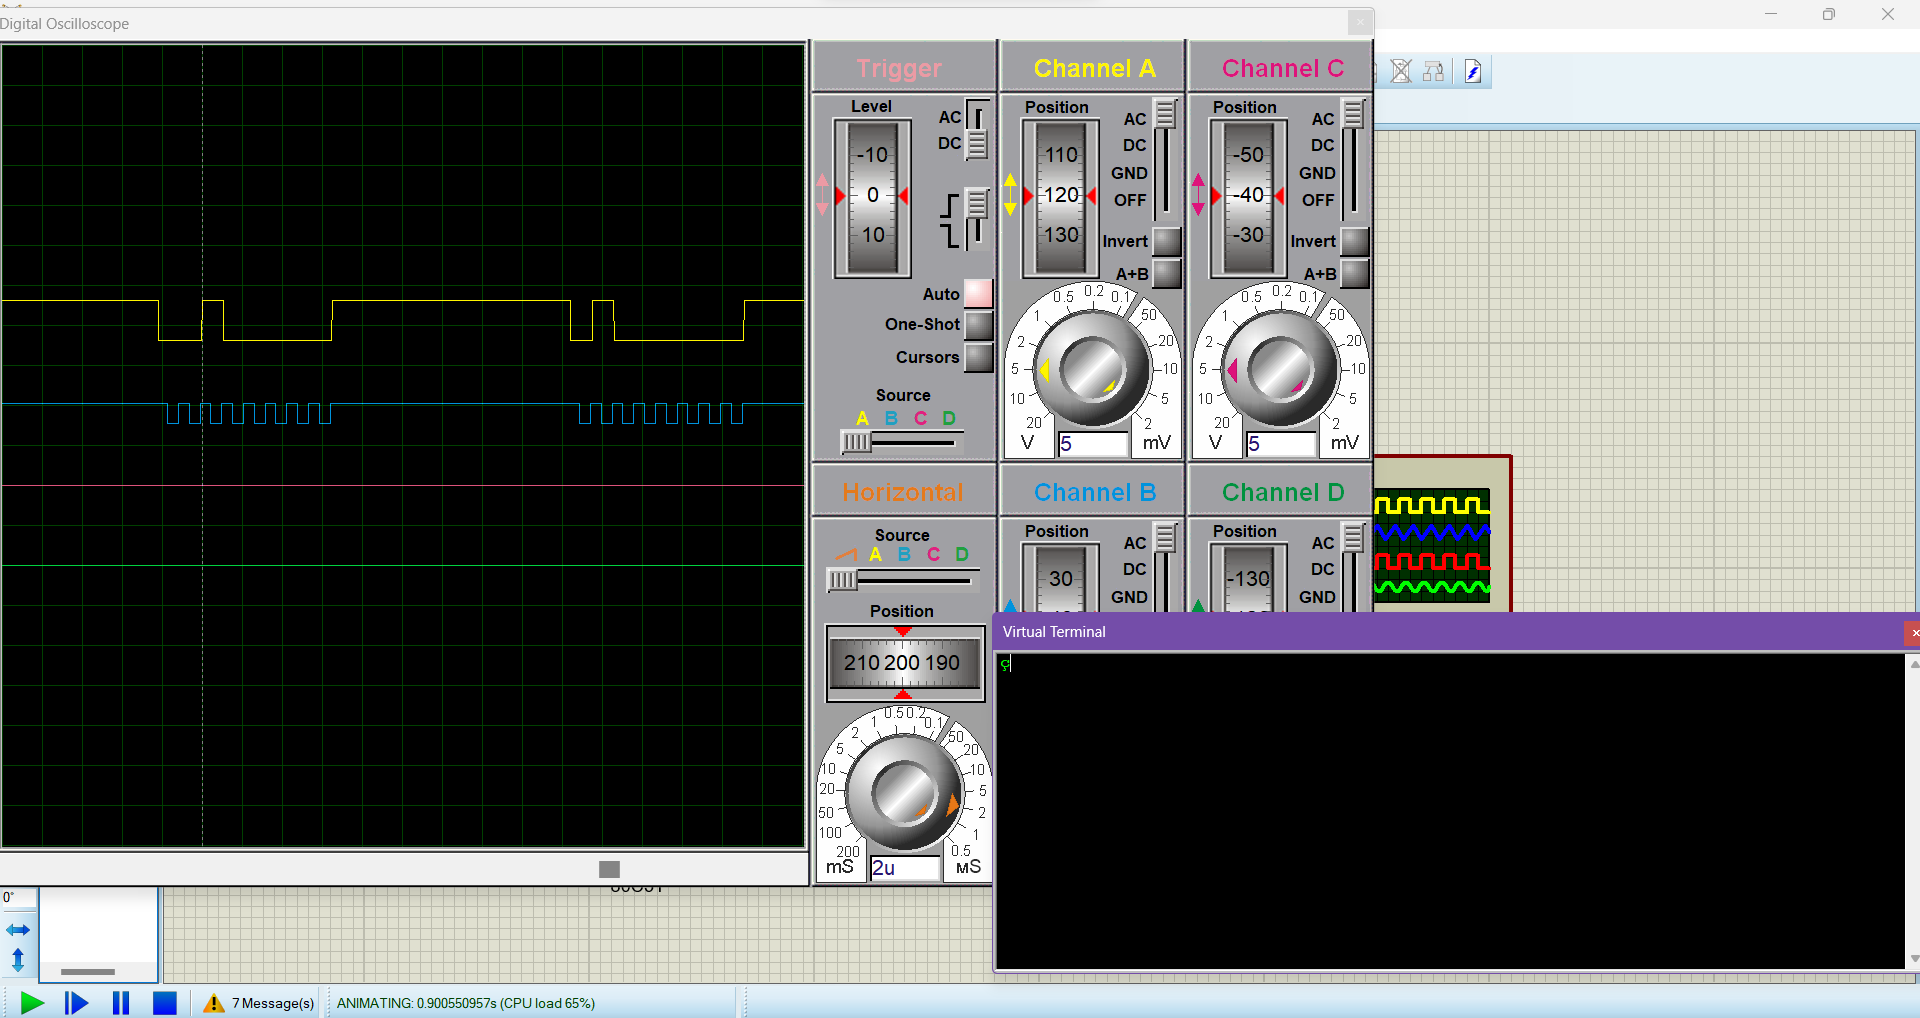
\includegraphics[width=0.48\linewidth]{result/p1_res.png}
		\captionof{figure}{نتیجه شبیه سازی}
	 \end{center}

	 برای محاسبه \texttt{baud-rate} از رابطه زیر استفاده میکنیم.

	 \begin{latin}
		\begin{eqnarray*}
			\text{baud-rate}&=&\text{clock freq.}\times\text{clock divider}
			\times\text{serial divider}\times\text{TH1 rate}\\
			&=& 
			\frac{11.0592\text{MHz}}{12\times32\times(255-TH_1+1)}=9600 \frac{Bits}{Sec}
		\end{eqnarray*}
	\end{latin}
\end{qsolve}

\end{document}

